\subsubsection{Experimento 1: Efecto de la variaci\'on de colores}
\par Para empezar con la experimentaci\'on relacionada a tiempos de ejecuci\'on correremos los distintos m\'etodos sobre un video con colores constantes y otro con colores variables y compararemos los resultados obtenidos. Esto nos va a servir a la hora de llevar a cabo otros experimentos, porque si los tiempos son similares entre un video y otro significa que los colores que elijamos para los distintos videos no van a influirnos en los tiempos de ejecuci\'on.

\par Vamos a crear un video que tiene resoluci\'on de 10px x 10px con un color fijo constante y otro video, de la misma resoluci\'on, pero con colores que oscilan de forma ordenada entre el blanco, el negro y sus tonos intermedios. Tomaremos bloques de 5 frames (podr\'iamos haber elegido cualquier n\'umero) y agregaremos 2 frames intermedios entre cada frame del video de entrada.


\subsubsubsection{Resultados del experimento 1}

\begin{figure}[ht]
	\begin{center}
		\subfigure [M\'etodo del Vecino mas cercano] {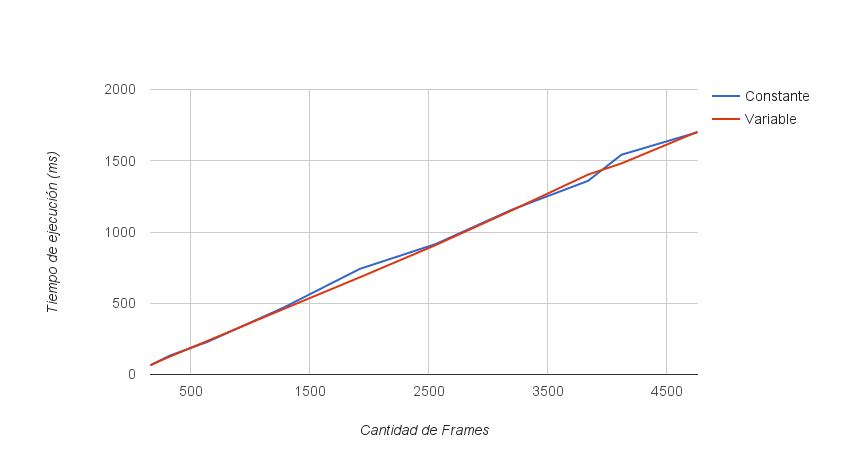
\includegraphics[width=0.70\columnwidth]{imagenes/tiempos/graf1_0.png}}
		\subfigure [M\'etodo Lineal] {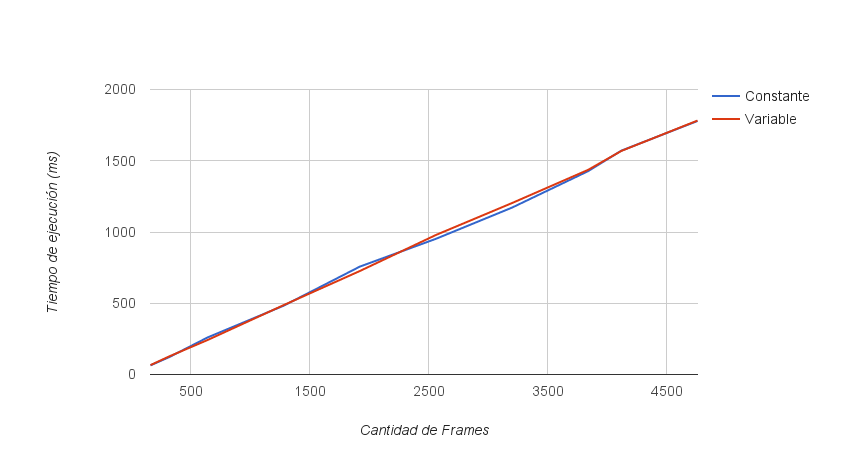
\includegraphics[width=0.49\columnwidth]{imagenes/tiempos/graf1_1.png}}
		\subfigure [M\'etodo de Splines naturales por bloques] {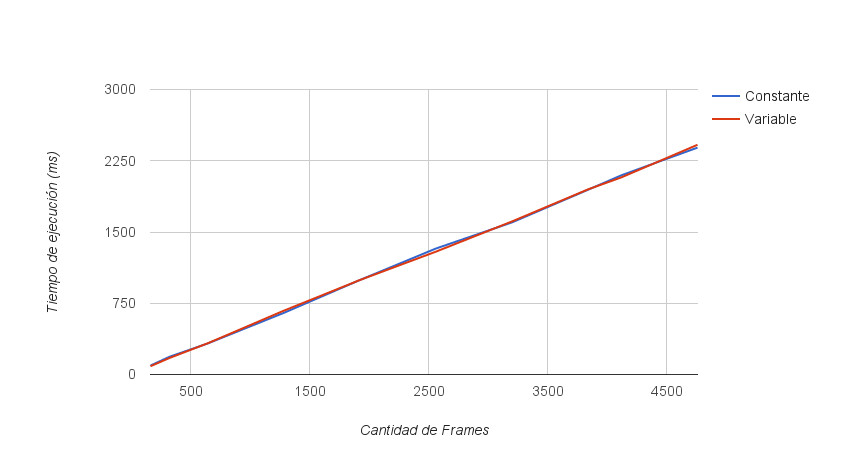
\includegraphics[width=0.49\columnwidth]{imagenes/tiempos/graf1_2.png}}
	\end{center}
\end{figure}


\par Como podemos observar en los gr\'aficos, los m\'etodos se comportan de la misma forma con ambas im\'agenes. Se notan diferencias en algunos momentos del m\'etodo del vecino mas cercano, pero manteniendo el mismo orden. No nos van a preocupar mucho estas diferencias, pero si las tendremos en cuenta de aqu\'i en adelante.
\par Luego de este experimento podemos asumir que el cambio de colores pr\'acticamente no va a influir en los tiempos de ejecuci\'on. Ahora s\'i podemos continuar con la experimentaci\'on teniendo en claro que ocurre con los colores.


\subsubsection{Experimento 2: Tiempos de ejecucí\'on vs Cantidad de Frames}
\par En este experimento vamos a comparar el tiempo de ejecuci\'on de los diferentes m\'etodos al aumentar la cantidad de frames de un video y tratar de determinar el orden de los mismos.

\par Para llevar a cabo el experimento vamos a crear videos con patrones de im\'agenes repetidos (tomando en consideraci\'on esos pequeños cambios que vimos en el experimento anterior) manteniendo el mismo ancho y alto de im\'agenes y cantidad de frames en aumento. La idea es fijar las variables de ancho (10px), alto (10px), variacion de colores (con un generador de patrones repetidos), frames intermedios (2) y tama~no de bloques (5)(para el caso del m\'etodo de Splines) para que no nos influyan en las mediciones y poder enfocarnos en la canidad de frames.

\subsubsubsection{Resultados del experimento 2}
\begin{figure}[ht]
	\begin{center}
		\subfigure [Tiempos de ejecuci\'on variando la cantidad de frames] {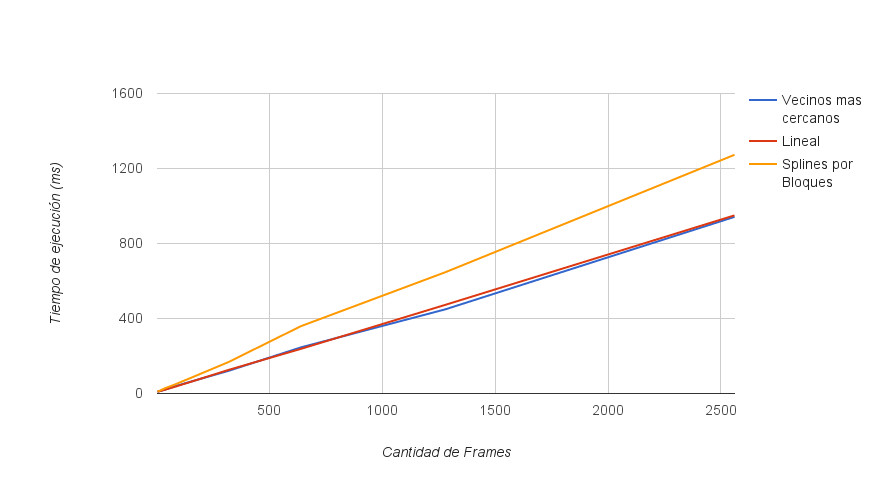
\includegraphics[width=0.9\columnwidth]{imagenes/tiempos/graf2.png}}
	\end{center}
\end{figure}
\par Luego de realizar el experimento podemos creer que el tiempo de ejecuci\'on de los tres m\'etodos es de orden lineal. Podemos notar que los Splines por Bloques se mantiene siempre por encima de los otros, pero mantienen su forma lineal. Mas adelante veremos las diferencias de calidad entre los m\'etodos y tendremos que tener en cuenta esta igualdad de orden, ya que no es tan grande como esper\'abamos en un principio. 

\paragraph{Cambios de inputs de entrada:}
De aquí en adelante realizaremos experimentos sobre 6 videos reales, con distintas calidades y duraciones. Los videos elegidos como inputs se encuentran en slow motion originalmente, y muestran situaciones que consideramos interesantes para analizar resultados cuantitativos y cualitativos, como por ejemplo, una pelota de tenis volando o fideos cayendo lentamente, ya que se pueden apreciar las diferencias con los videos originales más claramente.
\par A continuación una breve descripción de los videos de entrada que utilizamos para los tests: (de menor a mayor calidad)
\begin{multicols}{2}
\begin{itemize}
\item \textit{cupcake} : $\#$frames = 252, tamaño 240x360
\item \textit{perro} : $\#$frames = 252, tamaño 360x360
\item \textit{morocho} : $\#$frames = 452, tamaño 360x360
\item \textit{tenis} : $\#$frames = 450, tamaño 240x426
\item \textit{bebes} : $\#$frames = 225, tamaño 544x1280
\item \textit{fideos} : $\#$frames = 125, tamaño 720x1280
\end{itemize}
\end{multicols}


\subsubsection{Experimento 3: Tiempos de ejecucí\'on vs Tama\~no de Bloques}
\par Como tomamos la determinación de aplicar el m\'etodo de Splines de a bloques de frames, queremos medir cu\'anto nos afecta el tama\~no que decidamos darle a estos bloques en el tiempo de ejecuci\'on del m\'etodo.
\par Para esto vamos a tomar los videos antes mencionados, y correremos el m\'etodo de splines con diferentes tama\~nos de bloque. Mantendremos la cantidad de frames intermedios fija (2)y observaremos el comportamiento del m\'etodo.

\subsubsubsection{Resultados del experimento 3}
\begin{figure}[ht]
	\begin{center}
		\subfigure [Tiempos de ejecuci\'on variando el tamaño de los bloques] {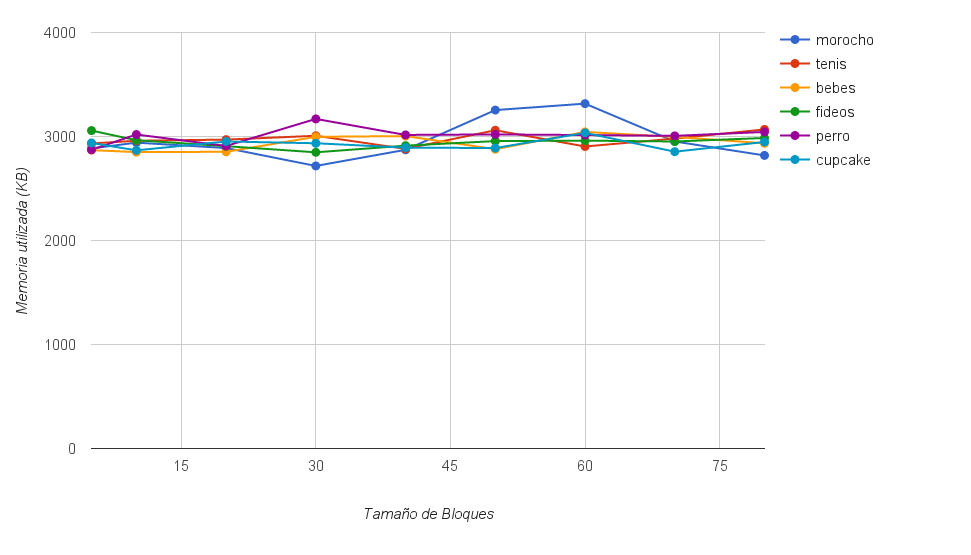
\includegraphics[width=1\columnwidth]{imagenes/tiempos/exp3_gabriel.png}}
	\end{center}
\end{figure}
\par Podemos observar que a pesar de algunas diferencias el orden del tiempo se mantiene constante y no se vi\'o afectado por el aumento del tama\~no de bloques. Nos parece normal que esto ocurra, ya que el algoritmo realiza la misma cantidad de pasos. La diferencia se ve en como se agrupan los datos, lo que si puede influir en las im\'agenes decididas a agregar como nuevos frames.
\par Estos tests fueron corridos en una computadora \textbf{DATOS RELEVANTES COMO MEMORIA RAM, PROCESADOR}. Al correr estos mismos tests en otras computadoras vimos diferentes resultados que expondremos en el siguiente experimento.

\subsubsubsection{Experimento 3 bis: Tiempos de ejecuci\'on vs Tama\~no de Bloques en computadoras con poca memoria}
\par Al llevar a cabo el experimento 3 nos vimos con complicaciones para correr los tests en una computadora. Planteamos las limitaciones de la computadora y pensamos que podr\'ia ser lo que afecta las mediciones.
\begin{itemize}
	\item En primer lugar, es una computadora con Pentium D (dos procesadores de 2.66GHz y 1024KB de memoria cache), lo que aument\'o los tiempos de ejecuci\'on en gran medida.
	\item En segundo lugar, cuenta con una memoria ram de 1.5 GB, por lo que creemos que al utilizar toda su memoria ram, pasar\'a a utilizar memoria mas lenta y eso puede influir fuertemente en los tiempos de ejecuci\'on.
\end{itemize}
\par Para abarcar el segundo item agregamos una medici\'on de memoria ram utilizada por el proceso. Vamos a ir consultando la memoria utilizada por el proceso y nos quedaremos con su valor m\'aximo, para as\'i tener una noci\'on de qu\'e puede estar pasando.

\subsubsubsection{Resultados del experimento 3 bis}
\begin{figure}[ht]
	\begin{center}
		\subfigure [Tiempos de ejecuci\'on enfocados en `cupcake', `morocho' y `tenis'] {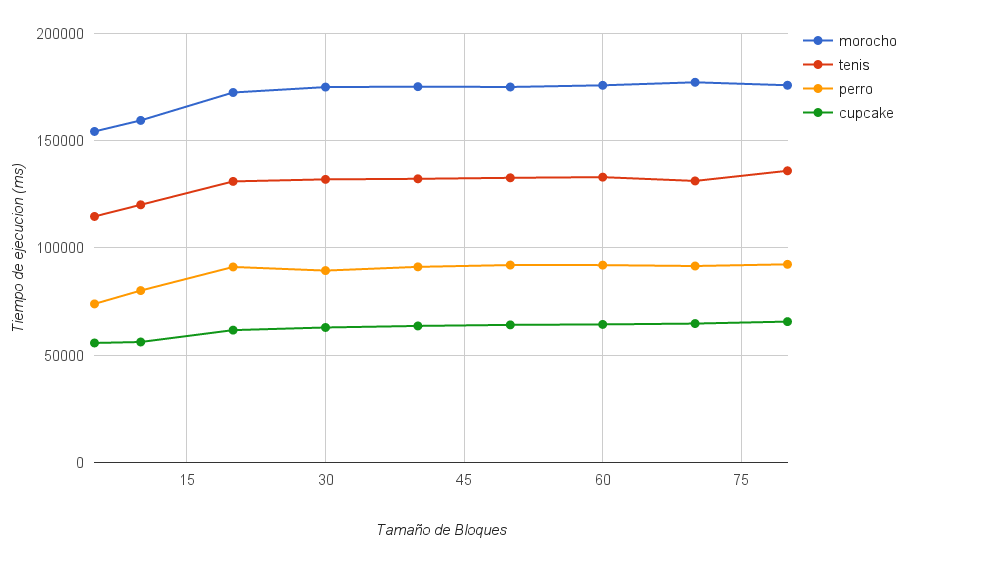
\includegraphics[width=1\columnwidth]{imagenes/tiempos/exp3_tiempos_normales.png}}
	\end{center}
\end{figure}
\FloatBarrier
\par En el caso de los tres videos con menor resoluci\'on (`cupcake', `morocho' y `tenis') obtenemos resultados del orden lineal, similares a los del experimento 3. Nombramos como dato importante la resoluci\'on ya que en memoria se guarda una matriz con los frames de un bloque (que su tama\~no va en aumento) y otras matrices y vectores que tambi\'en tienen al tama\~no de bloque entre sus medidas. Esta es la clave para entender el comportamiento de los otros dos videos (que mas adelante analizaremos).

\begin{figure}[ht]
	\begin{center}
		\subfigure [Memoria utilizada enfocado en `cupcake', `morocho' y `tenis'] {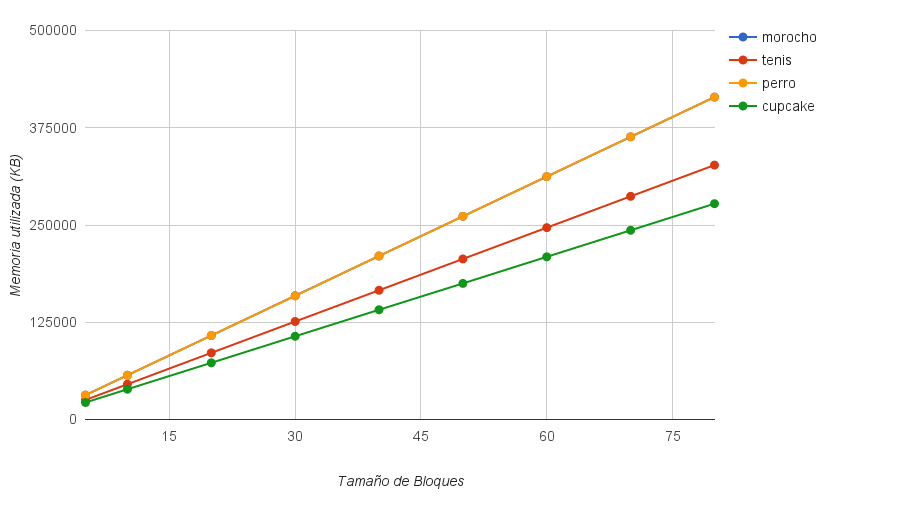
\includegraphics[width=1\columnwidth]{imagenes/tiempos/exp3_memoria_normales.png}}
	\end{center}
\end{figure}
\FloatBarrier
\par Con respecto a memoria utilizada, en los tres videos vemos un orden lineal en aumento, lo que es esperable por los detalles de la utilizaci\'on de memoria que comentamos anteriormente.

\begin{figure}[ht]
	\begin{center}
		\subfigure [Tiempos de ejecuci\'on de todos los videos] {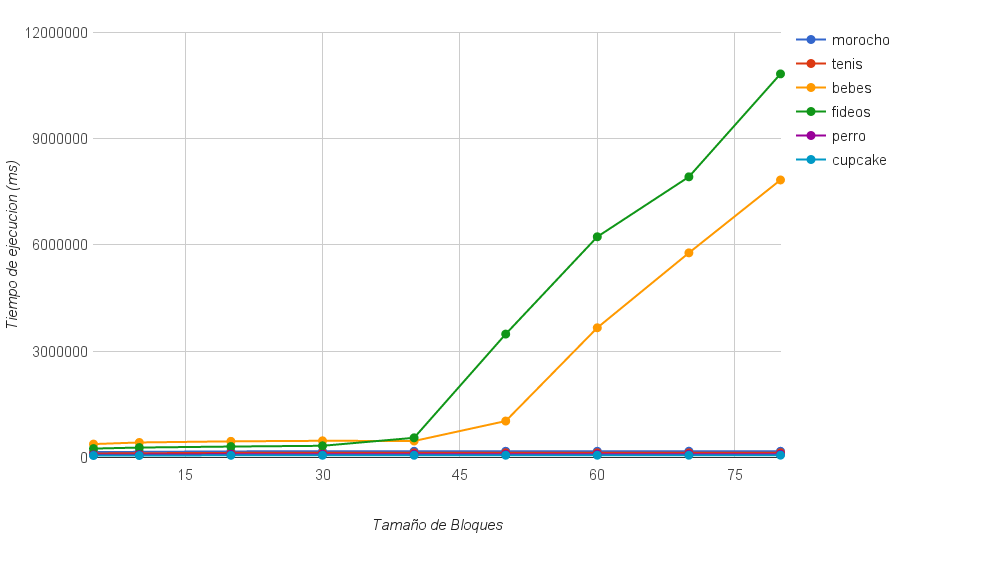
\includegraphics[width=1\columnwidth]{imagenes/tiempos/exp3_tiempos_todos.png}}
	\end{center}
\end{figure}
\FloatBarrier
\par Por parte de los videos `bebes' y `fideos' (los de mayor resoluci\'on) notamos que aumentan de forma lineal, pero con un grado mayor al resto. Luego, el video `fideos' al llegar a 30 comienza a aumentar de forma cuadr\'atica. Lo mismo sucede para el video `bebes' al llegar a 40. Para entender por qu\'e sucede esto veamos el gr\'afico de los resultados de utilizaci\'on de memoria de estos dos videos.
\begin{figure}[ht]
	\begin{center}
		\subfigure [Memoria utilizada por todos los videos] {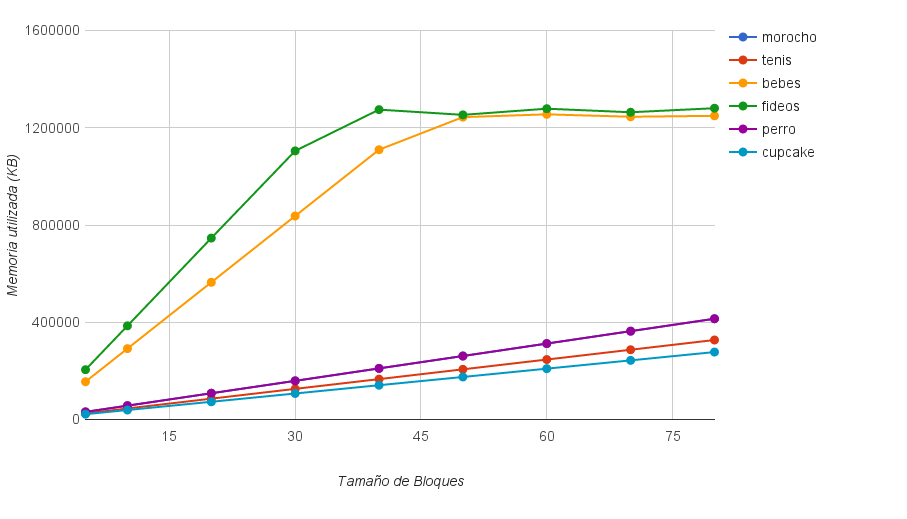
\includegraphics[width=1\columnwidth]{imagenes/tiempos/exp3_memoria_todos.png}}
	\end{center}
\end{figure}
\FloatBarrier
\par Podemos observar que para el video `fideos' la memoria ram utilizada va en aumento hasta llegar a valores cercanos a 1.2 GB (recordemos que la memoria de la computadora era de 1.5 GB) y luego se estanca en esos valores. Si tenemos en cuenta otros procesos que puedan estar ejecut\'andose en ese momento y un sistema operativo que controla la memoria y puede limitar su asignaci\'on, entendemos que al no poder utilizar mas memoria ram recurre a otras memorias de menor velocidad. Esto explica los tiempos de ejecuci\'on obtenidos a partir del tama\~no de bloque 30. Esto mismo sucede a partir del bloque 40 en el caso del video `bebes'.
\par Conclu\'imos que debemos tener en cuenta que el rendimiento del m\'etodo se ve fuertemente ligado a las caracter\'isticas de la computadora donde se corra. Igualmente para videos de calidad media y computadoras ligeramente modernas no observamos problemas.

\subsubsection{Experimento 4: Tiempos de ejecucí\'on vs Cantidad de frames intermedios}
\par Vamos a observar como se comportan los m\'etodos al variar la cantidad de frames que se desean agregar. A pesar de que no se hacen muchos pasos extra para agregar un frame intermedio y solo se realiza una ecuaci\'on, esta ecuaci\'on se repite para cada pixel del nuevo frame. Creemos que esto va a afectar mucho en el tiempo de ejecuci\'on de los tres m\'etodos.
\par Correremos los distintos m\'etodos sobre los 6 videos antes mencionados aumentando la cantidad de frames intermedios y observaremos como se comportan seg\'un sus diferentes caracter\'isticas.

\subsubsubsection{Resultados del experimento 4}
\begin{figure}[ht]
	\begin{center}
		\subfigure [M\'etodo del Vecino mas Cercano] {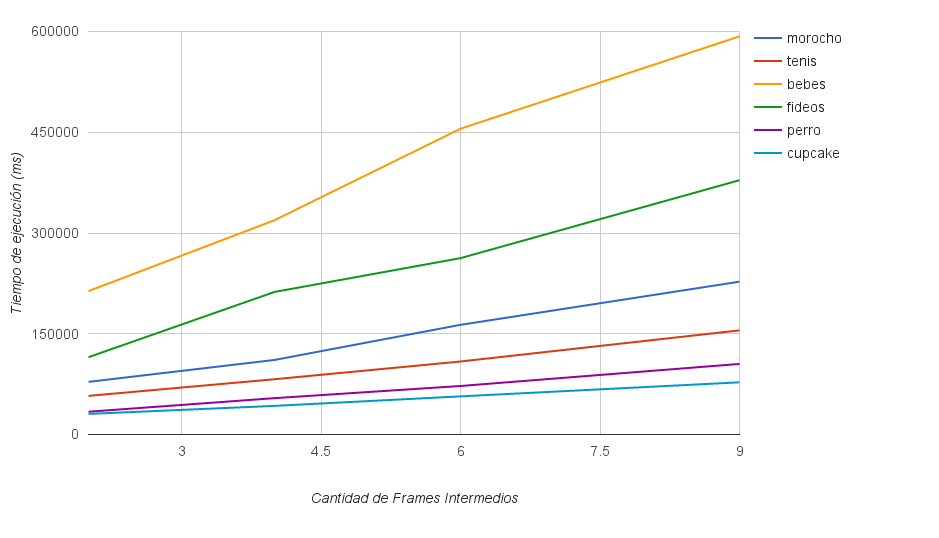
\includegraphics[width=0.9\columnwidth]{imagenes/tiempos/exp4_cercano.png}}
		\subfigure [M\'etodo Lineal] {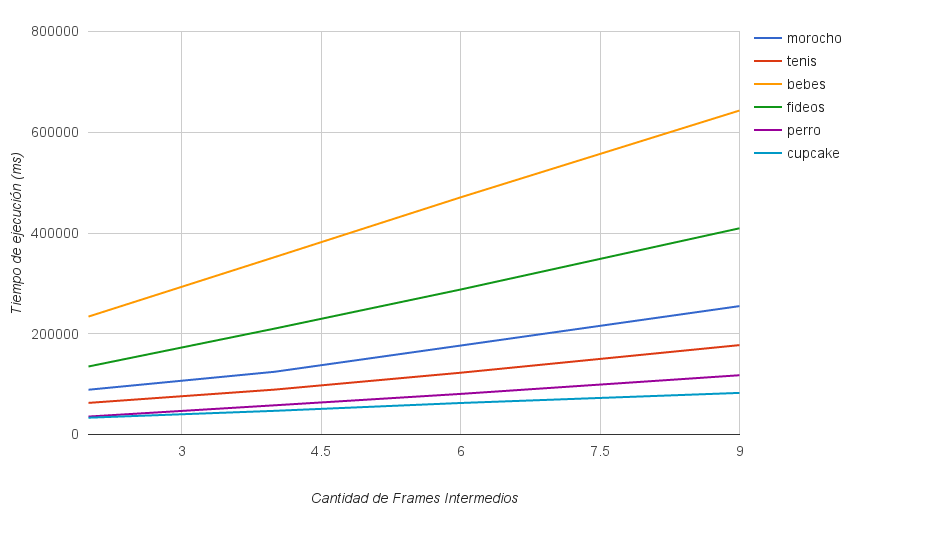
\includegraphics[width=0.49\columnwidth]{imagenes/tiempos/exp4_lineal.png}}
		\subfigure [M\'etodo de Splines Por Bloques] {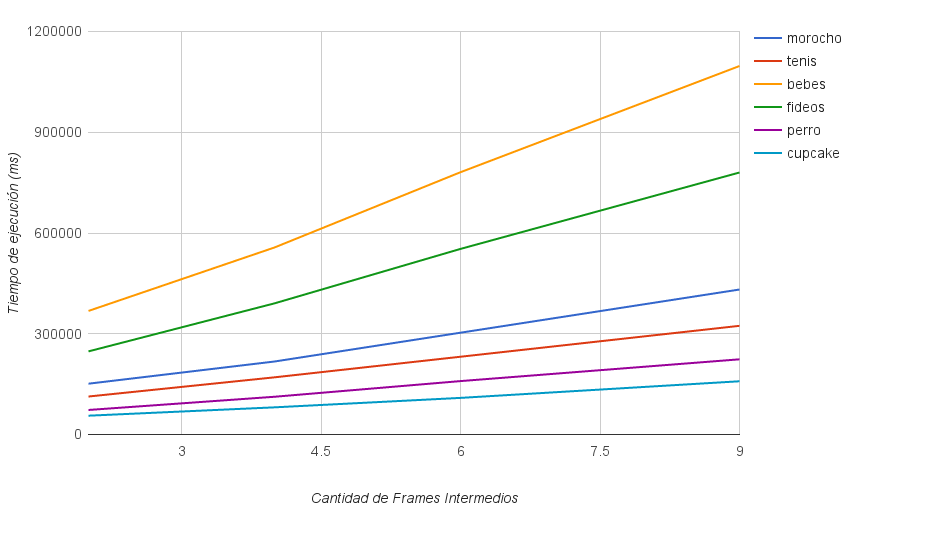
\includegraphics[width=0.49\columnwidth]{imagenes/tiempos/exp4_splines.png}}
	\end{center}
\end{figure}
\FloatBarrier

\par Al ver los resultados lo primero que notamos en un \'orden similar y lineal entre los videos Cupcake, Tenis, Perro, Morocho. Los videos Bebes y Fideos mantienen ordenes mayores. Esto se lo adjudicamos al hecho de que son los videos con mayor resoluci\'on, y se ven mas afectados al agregar frames. Igualmente mantienen un orden lineal dentro de lo esperado.

\par Veamos mas en detalle el efecto de agregar un frame. Supangamos que tomamos N como la cantidad de frames del video original y F como cantidad de frames intermedios a agregar. De esta forma al aplicar alguno de los m\'etodos se agregan F frames N-1 veces $\longrightarrow$ F*(N-1). Si aplicamos uno de los m\'etodo nuevamente, pero esta vez con F+1 frames intermedios, se agregar\'an F+1 frames N-1 veces $\longrightarrow$ (F+1)*(N-1) = F*(N-1) + (N-1). Con este razonamiento simple y sin entrar en detalles podemos convencernos de que al aumentar la cantidad de frames aumentamos de forma lineal la cantidad de operaciones a realizar (agregamos N-1 operaciones `agregar frame intermedio').